%
%  untitled
%
%  Created by Joan T. Matamalas Llodrà on 2011-04-19.
%  Copyright (c) 2012. All rights reserved.
%
\documentclass[10pt, journal]{IEEEtran}

% Use utf-8 encoding for foreign characters
\usepackage[utf8]{inputenc}

% Setup for fullpage use
\usepackage{fullpage}

% Uncomment some of the following if you use the features
%
% Running Headers and footers
%\usepackage{fancyhdr}

% Multipart figures
\usepackage{subfigure}

% More symbols
\usepackage{amsmath}
\usepackage{amssymb}
\usepackage{latexsym}

% Surround parts of graphics with box
\usepackage{boxedminipage}

% Multirow tables
\usepackage{multirow} 

% Package for including code in the document
\usepackage{listings}

% If you want to generate a toc for each chapter (use with book)
%\usepackage{minitoc}

% This is now the recommended way for checking for PDFLaTeX:
\usepackage{ifpdf}

%\newif\ifpdf
%\ifx\pdfoutput\undefined
%\pdffalse % we are not running PDFLaTeX
%\else
%\pdfoutput=1 % we are running PDFLaTeX
%\pdftrue
%\fi

\ifpdf
\usepackage[pdftex]{graphicx}
\else
\usepackage{graphicx}
\fi
\title{Supervised classification exercise\\Introduction to Machine Learning}
\author{Marc Oliu \& Joan T. Matamalas}

\date{\today}

\begin{document}

\ifpdf
\DeclareGraphicsExtensions{.pdf, .jpg, .png}
\else
\DeclareGraphicsExtensions{.eps, .jpg}
\fi

\maketitle

\begin{abstract}
Nulla vitae elit libero, a pharetra augue. Donec id elit non mi porta gravida at eget metus. Etiam porta sem malesuada magna mollis euismod. Cras justo odio, dapibus ac facilisis in, egestas eget quam. Nulla vitae elit libero, a pharetra augue. Nullam id dolor id nibh ultricies vehicula ut id elit.
\end{abstract}

\section{Introduction} % (fold)
\label{sec:introduction}
The problem of classifying a set of images with two possible classes by means of a binary classifier is a long studied problem which has many techniques for its resolution. The goal of this paper is to analyze the performance of three commonly used techniques for two distinct data sets with a varying number of features and different data distribution. More precisely, the algorithms will be run for a linearly separable dataset with 13 features, and for a non-linearly separable dataset with 34 features.\\

The three algorithms to be analyzed are the linear Support Vector Machine (SVM), a kernelized version of the Support Vector Machine using the Radial Basis Function kernel (RBF-SVM), and the Adaboost meta-classifier.\\

The SVM algorithm is a linear classifier which defines a delimiting vector to separate the two classes of the data. For this implementation, a soft-margin version of the classifier which allows for data with overlapping classes is used in order to prevent the algorithm from destabilizing in non-linearly separable data. The RBF-SVM algorithm is a kernelized version of the SVM which transforms the data to be classified by projecting the points into a new dimension by means of a radial basis function, which allows for a better separability of the data.\\

Finally, the Adaboost meta-classifier is used in conjunction with the linear SVM. The Adaboost (or adaptive boosting) is an algorithm consisting on the generation of a set of weighted weak models which then classify the data by means of a weighted voting of the results of the model. Multiple weak algorithms were considered for the meta-classifier, but finally SVM was chosen for being the one with the lowest out of sample error.
% section introduction (end)

\section{Specification of the problem} % (fold)
\label{sec:specification_of_the_problem}
The general algorithm of the problem consists on a 10-fold cross-validation of the test data sets to calculate the out of sample error for the used algorithms, and for each fold a 3-fold cross-validation is performed over the train data to select the parameters of the models. Three folds are used instead of 10 because of the computational cost of the system, but a 10-fold cross-validation would be preferred to increase the accuracy of the estimation of the out of sample error for the given parameters.\\

In this section the specification of each algorithm will be explained, as well as the general algorithm used for the obtention and analysis of the out of sample error.

\subsection{The Linear Support Vector Machine (SVM) algorithm} % (fold)
\label{sub:the_linear_support_vector_machine_svm_algorithm}
The SVM algorithm consists on the optimization of a hyperplane which is then used for the classification of the data. The two parameters which describe the hyperplane are its director vector, represented by W, and the offset of the hyperplane, represented by `b'.\\

The hyperplane resulting from the training of the model is then used as a separator between the two classes, where all elements which fall above the hyperplane belong to one of the classes, and the ones falling below belong to the other. These two classes are represented by a +1 and a -1 value correspondingly, which simplifies the training and classification tasks.\\

The equation \ref{eq:svm_maximize} represents the maximization function used to select the alpha values for the different support vectors in the dual form of the SVM with soft margin. The alpha values represent the weight of each support vector, and has a value between 0 and C, being C the parameter to optimize. A higher value for alpha means that a miss-classification of the related support vector is more heavily penalized, so increasing the value of C increases the maximum weight of each support vector.\\
\begin{equation}
	\begin{aligned}
		& \underset{\alpha_i}{\text{max}}
		& & L(\alpha) = \sum_{i=1}^{n}{\alpha_i} - \frac{1}{2}\sum_{i,j}\alpha_i\alpha_j y_i y_j k(x_i,x_j)\\
		& \text{s.t.}
		& & 0 \le \alpha_i \le C \land \sum_{i=1}^n{\alpha_i y_i} = 0
	\end{aligned}
	\label{eq:svm_maximize}
\end{equation}

Once the alpha values are optimized, the values for the director vector W of the hyperplane and its offset `b' are calculated out of the support vectors, considering as support vectors only those elements with a value above 0 for alpha, as it can be seen on the equations at figure \ref{eq:svm_wb}.\\
\begin{equation}
	\begin{aligned}
		&w = \sum_i{\alpha_iy_ix_i} = 0\\
		&b = \frac{1}{\#SV}\sum_{i \in SV}{y_i-(\sum_{m \in SV}{\alpha_my_mx_m\cdot x_i})}
	\end{aligned}
	\label{eq:svm_wb}
\end{equation}

Once the training of the model is completed, the classification of one element can be performed by using only the W and `b' parameters, which represent the model. To do so, the equation of figure \ref{eq:svm_classify} is used. What this equation does is to calculate the position of a data point with respect to the hyperplane and get the sign of the result. If the element is above the hyperplane, it belongs to the +1 class, and if below, to the -1 class.
\begin{equation}
	\mathbf{w}\cdot x + b
	\label{eq:svm_classify}
\end{equation}
% subsection the_linear_support_vector_machine_svm_algorithm (end)

\subsection{The Radial Basis Function kernelized SVM (RBF-SVM) algorithm} % (fold)
\label{sub:the_radial_basis_function_kernelized_svm_rbf_svm_algorithm}

The RBF-SVM algorithm is a variation of the SVM algorithm which uses a non-linear kernel different from the dot product of data points. In particular, the kernel used in this algorithm for the kernelized SVM is the radial basis function, which is calculated by using the function represented at figure \ref{eq:rbf_kernel}. As it can be seen in the function, there is an sigma parameter, which thefines the width of the gaussian distribution over the new dimension. As the sigma value increases, the gaussian form is wider, while it gets sharper as sigma decreases.\\
\begin{equation}
	k_{rbf}(x_1,x_2) = e^\frac{||x_1-x_2||^2}{2\sigma^2}
	\label{eq:rbf_kernel}
\end{equation}
The kernel functions allow for the calculation of the dot-product between two points in a higher dimensional space without the need of first increasing the dimensionality of the data points, simplifying the process of optimizing the function, since the same optimization function seen in the previous section (figure \ref{eq:svm_maximize}) is valid, needing only to replace the dot product by the kernel function.\\

Since the dot product is performed on the lower-dimensional data, and the dataset isn't transformed to the higher-dimensional space, it's not possible to calculate the hyperplane director vector from the support vector, and thus the support vectors, their alphas and labels must be added to the model in order to classify other data points. The `b' value, which represents the offset of the hyperplane, is calculated in the same way as with the linear SV, as seen in the second function of figure \ref{eq:svm_wb}.\\

To classify the new instances, the equation seen at figure \ref{eq:rbf_classify} is used. This equation first calculates the position of the data point with respect to the hyperplane without taking into account the offset by using directly the support vector, and then adds the offset to the result. This is the same procedure used in the normal SVM, but since now the equation of the hyperplane isn’t defined, the support vectors that define this hyperplane are used directly to check the position of the new data point with respect to the hyperplane.\\

\begin{equation}
	\sum_{i+1}{\alpha_{i}y_i k(x_i,x)}
	\label{eq:rbf_classify}
\end{equation}

As with the SVM models, the sign of the result defines the class of the data point.
% subsection the_radial_basis_function_kernelized_svm_rbf_svm_algorithm (end)

\subsection{The Adaboost Algorithm} % (fold)
\label{sub:the_adaboost_algorithm}
The adaboost algorithm is a meta-classifier that uses a linear combination of weak classifiers of the same type to classify a data point, as it can be seen in figure \ref{eq:ada_classify}. As it can be seen, each weak classifier as a weight assigned, which is inversely proportional to the classification error of the weak model.\\
\begin{equation}
	H(x) = sign(\sum_{t=1}^{T}{\alpha_t h_t(x)})
	\label{eq:ada_classify}
\end{equation}

An weak classifier can be used with the adaboost algorithm, and some have been considered for this work. More specifically, the threshold, perceptron and linear SVM classifiers have been considered for being used with the adaboost algorithm. Finally the selected one has been the SVM algorithm, since it is the one with the highest predictive power, and because it’s a good option to check the improvement of the Adaboost algorithm over the normal SVM classifier.\\

\begin{equation}
	\begin{aligned}
	&D_{t+1}(i) = \frac{D_t(i)e^{-\alpha_ty_th_t(x_i)}}{Z_t}\\
	&Z_t = \sum_{i}{D_t(i)e^{\alpha_ty_th_t(x_i)}}
	\end{aligned}
	\label{eq:updweights}
\end{equation}

The training of the adaboost algorithm is performed in a cyclic way, where at the beginning the weights of each data point to classify are all set to the same value 1/N, and on each iteration a new model is generated and weighted by following the formula seen at figure \ref{eq:ada_alpha}, and the weights are updated for the misclassified data points on the new model by following the function \ref{eq:updweights}, normalizing the weights afterwards.

\begin{equation}
	\alpha_t = \frac{1}{2}log\frac{1-\epsilon}{\epsilon}
	\label{eq:ada_alpha}
\end{equation}

% subsection the_adaboost_algorithm (end)

\subsection{Main algorithm} % (fold)
\label{sub:main_algorithm}
The main algorithm used to run the experiment consists on a 10-fold cross-validation over the data set, performing an optimization of the parameters of each model at each one of the folds, by performing a 3-fold of the training data.\\

First the data is divided into 10 folds, and an iteration over the folds selects one fold at each iteration to estimate the out of sample error of the models to generate. Then, the remaining ten folds are used to train the three models. These remaining 9 folds are merged into three folds, and a new iteration over the three folds is performed, selecting one fold at each iteration, which will be used to estimate the error of the tested parameters.\\

The two training folds are used to train the three kinds of models for different values of the parameters, and the out of sample error for the selected values is estimated from the other fold. Once the out of sample error has been calculated from the three folds, the errors for each model type and set of parameters are averaged, and the set of parameters for each model that gives the lowest mean of out of sample errors are selected. Then the models are trained with t	he data of the three folds (which is the data of the 9 training folds of the main 10-fold cross-validation) and the selected parameters.\\

Finally, the out of sample errors tested for the optimal parameters at each fold of the 10-fold cross validation are averaged for each model, giving the mean out of sample error. Also, the standard deviation and confidence intervals are calculated for the ten folds.\\

As for the error surface, it’s obtained by averaging the error surfaces of each fold of the 10-fold cross-validation, which in turn are obtained as the average of the error surfaces for the 3-fold cross validation performed at each fold.\\
% subsection main_algorithm (end)

% section specification_of_the_problem (end)

\section{Organization of the software} % (fold)
\label{sec:organization_of_the_software}
To implement the algorithms described above, the Matlab IDE has been used. The code has been distributed between a main script file named ‘main.m’ and a series of functions which implement the different functionalities of the algorithms.\\

The main.m script is used to select the dataset to be used for the analysis, which is then handled to the crossValidate function, which implements the cross-validation algorithm described before. The resulting data structure of this function is then both saved to a variable in the workspace and to a matlab file at disk.\\

The implemented functions are listed below, with a brief explanation of the task they perform:

\begin{itemize}
\item parser\_arff: Parses a file containing a matrix. This parser takes a text file and process it, removing the comments and type declarations and parsing the remaining matrix. The format of the matrix is expected to be a row per line, separated by commas. The last column (classes) is converted to numerical values, and an ordered list of the original class names is returned.
\item parser\_nfold: Parses both the train and test datasets for a specific fold of the given dataset, which is passed by its name, by using the parser\_arff function.
\item crossValidate: Runs the core of the experiment, performing a 10-fold cross-validation of the data set by training the models at each fold, selecting their optimal parameters at each fold. It returns the out of sample error for each model, its statistics and the error surface for the input parameters of the models.
\item train\_svm: Train a SVM with the given data, class labels, and value of C (alphas upper bound). If a fourth parameter sigma is given, an RBF-SVM is performed.
\item test\_svm: Given a test dataset and a model generated by the train\_svm function, classify the instances of the test dataset.
\item train\_adaboost: Train an adaboost model with the given data and class labels, and a maximum of T iterations. An optional fourth parameter can be passed to indicate the type of weak classifiers to use. If nothing is passed, the SVM model will be used for the weak classifiers.
\item train\_perceptron: Train a linear perceptron with the given data and labels, returning the resulting model.
\item test\_perceptron: Given a data set and a model generated when a perceptron algorithm is trained, classifies the instances of the data set, returning a vector of classes.
\item train\_perceptronSigmoid: Trains a perceptron with the given data and labels which implements a sigmoidal function.
\item test\_perceptronSigmoid: Classifies the given data set by using the passed sigmoidal perceptron model, returning a vecor of labels with the result of the classification,
\item sus: Impelements a stochastic universal sampler which, given a set of individuals, their corresponding classes as a vector of labels, and their corresponding probabilities as a vector of weights, returns a subset of the passed individuals and their corresponding labels.
\item rbfKernel: Calculates the RBF kernel for the RBF-SVM classifier. It returns a matrix with the kernel of all combinations of individuals from one vector with the members of the second vector, for the given sigma parameter.
\item linearKernel: Calculates the dot product of instances for the linear SVM classifier. It returns a matrix with the dot product of all combinations of individuals from one vector with the members of the second vector.
\end{itemize}

% section organization_of_the_software (end)


\section{Experiments} % (fold)
\label{sec:experiments}

\subsection{Ionosphere dataset} % (fold)
\label{sub:ionosphere_dataset}

% subsection ionosphere_dataset (end)

\subsection{Heart-statlog dataset} % (fold)
\label{sub:heart_statlog_dataset}

\begin{figure}[ht!]
	\centering
	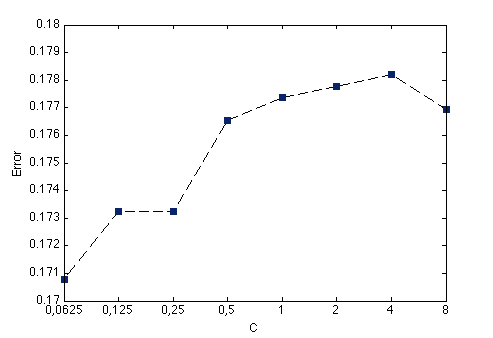
\includegraphics[width=0.5\textwidth]{img/errorSVMHeartLog}
	\caption{Linear SVM parameter error}
	\label{fig:errorSVMHeartLog}
\end{figure}


\begin{figure}[ht!]
	\centering
	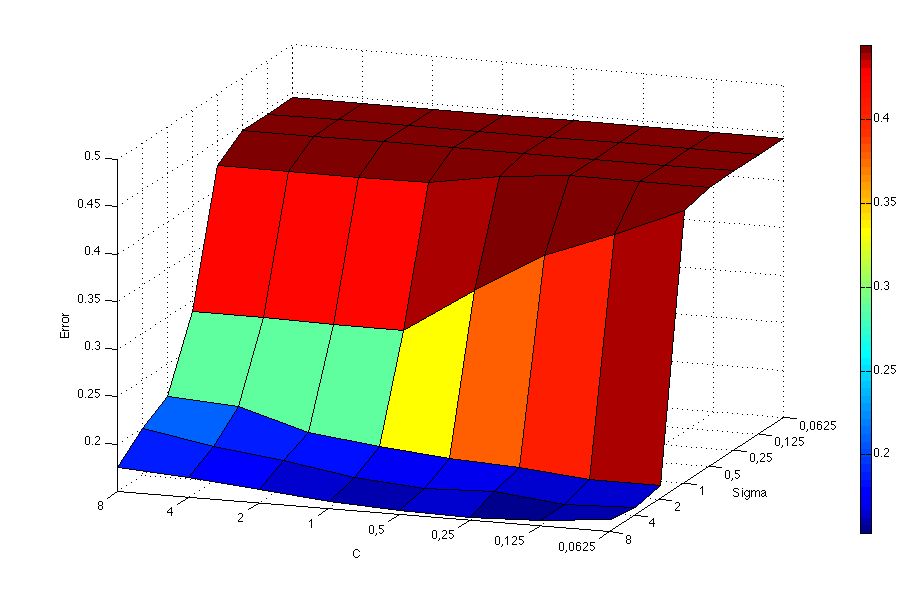
\includegraphics[width=0.5\textwidth]{img/errorSurfaceHeartStatLog}
	\caption{RBF parameters error surface for the heart-statlog dataset}
	\label{fig:errorSurfaceHeartStatLog}
\end{figure}


\begin{table}[ht!]
	\centering
	\begin{tabular}{|c|c|c|c|c|}
		\hline
		\textbf{Algorithms} & \textbf{Mean} & $\mathbf{\sigma}$ & \textbf{SEM} & \textbf{C.I.}\\\hline
		SVM & 0.1667 & 0.0586 & 0.0185 & $\pm$0.0419\\\hline
		RBF & 0.1667 & 0.0501 & 0.0159 & $\pm$0.0359\\\hline
		ADA & 0.1630 & 0.5 & 0.0158 & $\pm$0.0358\\\hline
	\end{tabular}
	\label{tab:heartErrorComparison}
	\caption{Heart-stat log error results}
\end{table}

\begin{figure}[ht!]
	\centering
	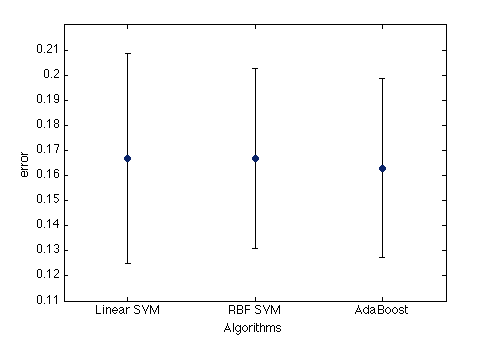
\includegraphics[width=0.5\textwidth]{img/heartLogAnalisy}
	\caption{Error and confidence interval}
	\label{fig:heartLogAnalisy}
\end{figure}


\begin{table}[ht!]
	\centering
	\begin{tabular}{|c|c|c|}
		\hline
		\textbf{Test} & \textbf{p-value} & \textbf{Significative difference}\\\hline
		Linear-SVM \emph{vs} RBF-SVM & 1 & —\\\hline
		Linear-SVM \emph{vs} AdaBoost & 1 & —\\\hline
		RBF-SVM \emph{vs} AdaBoost & 1 & —\\\hline
	\end{tabular}
	\label{tab:heartWilcoxonTest}
	\caption{Wilcoxon statistical test}
\end{table}


% subsection heart_statlog_dataset (end)
% section experiments (end)

\section{Conclusions} % (fold)
\label{sec:conclusions}
From the results obtained by applying the three binary classification methods to the two data sets, it can be seen that in both cases the adaboost algorithm, which generates a model based on a weighted polling over various specialized linear SVM models, performs slightly better than in the case of a linear SVM model.\\

This is due to the non-linearity of the data in one case, where the out of sample error gets reduced by a 11\% on average, and due to the data not being completely linearly separable in the other, which makes it is impossible for an SVM classifier with soft margins to always classify the data correctly. On the other hand, the use of multiple SVM models in the poll when using adaboost, allows for the definition of non-linear boundaries between the classes, which reduces the number of missclassifications.\\

It can also be seen during the analysis that in the case of the adaboost classifier the accuracy of the model doesn't change when increasing the number of iterations T of the meta-classifier generation. This is due to the algorithm choosing always a low number of weak models, not getting better results by increasing the number of weak models above 3, and stopping the addition of new ones after the error of these models gets above 0.5. For that reason, even though the number of weak models is allowed to go above 3, no new models are added passed this value to prevent worsening the predition power of the model.\\

When comparing the results of the non-linear data set, it can be seen that the RBF-SVM algorithm outperforms both adaboost and SVM, by getting a 6.56\% mean out of sample error, while the other two get a 13.11\% and 12.54\% respectively. This behaviour is to expect, since the RBF-SVM models allow the classification in non-linear egions of the data space, while the other two types of models only work well when detecting lineal or curved separations between classes.\\

In the linear data set with some overlapping of the classes, on the other hand, it can be seen that both the SVM and RBF-SVM models have the same mean accuracy, with little difference on its standard deviation. This is because in the case of linearly separable data, the RBF-SVM separates the data with an hyperplane very similar to that of the linear SVM model. In the case of the Adaboost algorithm, which uses the linear SVM as weak classifier, the result is again very close to that of both SVM and RBF-SVM models, since a single SVM perceptron can correctly classify most of the cases the Adaboost algorithm classifies.\\

TODO: Analisis del cost computacional?
% section conclusions (end)

\section{Future Work} % (fold)
\label{sec:future_work}
The procedure could be repeated by implementing a 10-fold cross-validation when selecting the parameters of the model instead of the 3-fold cross-validation used in this paper. This would increase the accuracy of the error surfaces and the out of sample errors of the models.\\

Also other non-linear models can be tested to compare their accuracy with that of the RBF-SVM models. An interesting model to compare would be the K Nearest Neighbors model, since it works by polling the class of the neighboring data points, and as such is less sensitive to regions with overlapping data, being able to classify the new instances to the most representative class of the region.\\

Finally other types of kernels could be tried for the non-linear SVM in order to check their performances over different data distributions.\\
% section future_work (end)

\bibliographystyle{plain}
\bibliography{}
\end{document}
